\documentclass[12pt,a4paper]{report}

% --- Packages ---
\usepackage[utf8]{inputenc}
\usepackage[french]{babel}
\usepackage[T1]{fontenc}
\usepackage{graphicx}
\usepackage{geometry}
\geometry{margin=1.8cm}
\usepackage{hyperref}
\usepackage{amsmath,amssymb}
\usepackage{setspace}
\usepackage{titlesec}
\usepackage{array}
\usepackage{caption}
\usepackage{subcaption}
\usepackage{float}
\usepackage{xcolor}
\usepackage{colortbl}

% Définition de la couleur bleue exacte du modèle de Mariem Cherif pour le titre de couverture
\definecolor{mariemblue}{RGB}{0, 0, 255}

% Liens hypertexte en noir pour la table des matières et le corps du document
\hypersetup{
    colorlinks=true,
    linkcolor=black,
    citecolor=black,
    filecolor=black,
    urlcolor=black,
    pdftitle={Rapport de Projet de Fin d'Année - BioPulse},
}

\onehalfspacing

\begin{document}

% ==========================================
% PAGE DE GARDE / COVER PAGE (TAILLES EXACTES DE LOGOS SOUHAITÉES)
% ==========================================
\begin{titlepage}
    \centering
    
    % En-tête : Logo ISTIC 3.5cm à gauche, Texte Officiel au centre, Logo Carthage 3.5cm à droite
    \begin{minipage}{0.28\textwidth}
        \begin{flushleft}
            
\includegraphics[height=3.5cm]{images/istic_logo.png}
        \end{flushleft}
    \end{minipage}
    \hfill
    \begin{minipage}{0.42\textwidth}
        \centering
        \small
        \textbf{République Tunisienne}\\[0.02cm]
        \textbf{Le Ministère de l'Enseignement Supérieur}\\
        \textbf{et de la Recherche Scientifique}\\[0.05cm]
        \textbf{L'Université de Carthage}\\[0.05cm]
        \textbf{L'Institut Supérieur des Technologies de l'Information}\\
        \textbf{et de la Communication}
    \end{minipage}
    \hfill
    \begin{minipage}{0.28\textwidth}
        \begin{flushright}
            
\includegraphics[height=3.5cm]{images/carthage_logo.png}
        \end{flushright}
    \end{minipage}
    
    \vspace{0.4cm}
    
    {\Large \textbf{RAPPORT DE PROJET DE FIN D'ANNÉE}}\\[0.2cm]
    {\small \textbf{Soumis en vue de l'obtention du}}\\[0.1cm]
    {\large \textbf{DIPLÔME DE LICENCE EN SYSTÈMES EMBARQUÉS ET IOT}}\\[0.2cm]
    {\large \textbf{Parcours : Systèmes Embarqués et IoT}}\\[0.4cm]
    
    % Encadré du titre (Lignes bleues/noires + texte bleu comme le modèle de Mariem)
    \rule{\linewidth}{1.5pt} \\[0.2cm]
    { \Large \bfseries \color{mariemblue} Système de Pointeuse Biométrique Connectée avec Plateforme Web de Gestion Temps Réel (BioPulse) } \\[0.2cm]
    \rule{\linewidth}{1.5pt} \\[0.4cm]
    
    % Section Auteur
    {\normalsize \emph{Rédigé par :}}\\[0.05cm]
    {\large \textbf{MOHAMED DHIA CHAOUCH}}\\[0.3cm]
    
    % Section Entreprise (KSI) + Logo officiel KSI (4.5cm)
    {\normalsize \emph{Réalisé au sein de KSI}}\\[0.15cm]
    
\includegraphics[height=4.5cm]{images/ksi_logo.png}\\[0.2cm]
    
    % Superviseur & Signature
    {\normalsize \textbf{Superviseur professionnel : M. Ala JAOUACHI}}\\[0.15cm]
    {\normalsize \textbf{Signature :}}\\[0.4cm]
    
    \vfill
    
    {\large \textbf{Année Universitaire : 2025-2026}}
\end{titlepage}

% ==========================================
% DÉDICACES (ÉCRITURE AGRANDIE EN \large)
% ==========================================
\chapter*{Dédicaces}
\addcontentsline{toc}{chapter}{Dédicaces}

{\large
À mes chers parents, dont l'amour inconditionnel, les sacrifices et le soutien constant ont été ma source de force et d'inspiration tout au long de mon parcours académique et personnel.

\vspace{0.8cm}
À mes chers amis et collègues, pour leur présence rassurante, leurs encouragements inébranlables et les moments partagés qui ont enrichi cette expérience.

\vspace{0.8cm}
À toutes les personnes qui m'ont soutenu de près ou de loin, je vous exprime ma plus profonde gratitude et mon sincère respect.
}

\newpage

% ==========================================
% REMERCIEMENTS (ÉCRITURE AGRANDIE EN \large)
% ==========================================
\chapter*{Remerciements}
\addcontentsline{toc}{chapter}{Remerciements}

{\large
Je tiens à exprimer ma profonde et sincère gratitude à toute l'équipe de l'entreprise \textbf{Kernel Solutions and Innovation (KSI)} pour leur accueil chaleureux, leur bienveillance et la mise à disposition d'un environnement de travail stimulant tout au long de cette période de stage.

\vspace{0.8cm}
Je souhaite adresser mes remerciements les plus respectueux à mon encadrant professionnel, \textbf{M. Ala JAOUACHI}, pour sa disponibilité, ses conseils avisés, son expertise technique et son accompagnement précieux lors du développement de ce projet.

\vspace{0.8cm}
Je remercie également l'ensemble des enseignants et membres du corps administratif de l'\textbf{Institut Supérieur des Technologies de l'Information et de la Communication (ISTIC)} pour la qualité de l'enseignement dispensé et leur soutien durant mon parcours universitaire.
}

\newpage

% ==========================================
% TABLES DES MATIÈRES ET FIGURES (TEXTE NOIR)
% ==========================================
\tableofcontents
\newpage
\listoffigures
\newpage
\listoftables
\newpage

% ==========================================
% INTRODUCTION GÉNÉRALE
% ==========================================
\chapter*{Introduction générale}
\addcontentsline{toc}{chapter}{Introduction générale}

Dans un monde professionnel moderne en pleine transformation numérique, la gestion automatisée du temps de présence est devenue un enjeu majeur pour les entreprises et institutions. Les méthodes traditionnelles basées sur le pointage manuel sur papier ou des fiches de présence présentent des vulnérabilités, notamment les risques de fraude, les erreurs de saisie et la difficulté de centraliser les données en temps réel. Pour répondre à ces défis, l'intégration des technologies de l'Internet des Objets (IoT) et de la biométrie offre une alternative robuste, précise et automatisée.

\vspace{0.3cm}
Ce projet s'inscrit dans ce contexte et vise à concevoir et réaliser une pointeuse biométrique intelligente (basée sur un microcontrôleur ESP32 et un capteur d'empreintes digitales) connectée à une plateforme web de gestion en temps réel (développée avec Node.js, Express, MongoDB et React). Le système permet d'authentifier les employés par leurs empreintes digitales, de communiquer de manière résiliente via Wi-Fi ou Ethernet (protocole UDP et HTTP), et d'offrir un tableau de bord analytique complet dédié exclusivement au suivi rigoureux des présences, des retards et des absences.

\vspace{0.3cm}
Ce rapport est structuré en quatre chapitres principaux :
\begin{itemize}
    \item Le \textbf{Premier Chapitre} présente le cadre général du projet, l'organisme d'accueil KSI, la problématique, la solution proposée ainsi que la méthodologie de travail adoptée.
    \item Le \textbf{Deuxième Chapitre} est consacré à l'étude du projet, détaillant l'analyse des besoins fonctionnels et non-fonctionnels, la modélisation UML et la conception logicielle/matérielle.
    \item Le \textbf{Troisième Chapitre} décrit la réalisation du système, incluant l'environnement de développement, le câblage électronique des composants matériels, la programmation du firmware ESP32 et le développement de la plateforme web.
    \item Le \textbf{Quatrième Chapitre} traite d'un module d'extension et de résilience du système (découverte automatique UDP du serveur, gestion des erreurs de connexion, bascule réseau Ethernet/Wi-Fi et synchronisation), suivi de la présentation des résultats obtenus.
\end{itemize}

\newpage

% ==========================================
% CHAPITRE 1 : CONTEXTE DU PROJET
% ==========================================
\chapter{Contexte du projet}

\section{Introduction}
Dans ce premier chapitre, nous présentons le cadre général dans lequel s'inscrit notre projet de fin d'année. Nous commençons par une présentation détaillée de l'entreprise d'accueil, \textbf{Kernel Solutions and Innovation (KSI)}. Ensuite, nous exposons la situation problématique ayant motivé ce travail, analysons les solutions existantes à travers une étude de l'état de l'art, et décrivons la solution proposée. Enfin, nous présentons la méthodologie de travail adoptée (Agile / Kanban) ainsi que la planification temporelle des tâches réalisées.

\section{Organisme d'accueil}
\textbf{Kernel Solutions and Innovation (KSI)} est une société de services et d'ingénierie informatique spécialisée dans le développement de solutions technologiques innovantes. L'entreprise accompagne aussi bien les entreprises commerciales que les institutions en leur fournissant des services d'ingénierie logicielle sur mesure, d'intégration de systèmes IoT et de conseil technologique.

\begin{figure}[H]
    \centering
    \IfFileExists{images/ksi_logo.png}{
\includegraphics[width=0.35\textwidth]{images/ksi_logo.png}}{\textbf{[Logo KSI]}}
    \caption{Logo de KSI.}
    \label{fig:ksi_logo}
\end{figure}

Grâce à une équipe d'ingénieurs qualifiés, KSI se distingue par sa capacité à concevoir des solutions performantes, évolutives et adaptées aux besoins spécifiques de ses clients. Les principaux domaines d'activité de l'entreprise comprennent :
\begin{enumerate}
    \item \textbf{Développement de logiciels sur mesure :} Conception d'applications web, mobiles et embarquées intuitives et performantes.
    \item \textbf{Services de maintenance et de support :} Suivi post-déploiement, mises à jour technologiques et assistance technique continue.
    \item \textbf{Conseil technologique et IoT :} Accompagnement stratégique, intégration de systèmes matériels/logiciels et optimisation des infrastructures IT.
\end{enumerate}

\section{Présentation du projet}
L'objectif de ce projet est de concevoir et de développer un système complet et intelligent de gestion du temps de présence, baptisé \textbf{BioPulse}. Ce système combine un terminal matériel autonome (pointeuse biométrique basée sur le microcontrôleur ESP32, un capteur d'empreintes digitales Adafruit, un écran graphique LCD ILI9341, un pavé numérique et un double contrôleur réseau Ethernet/Wi-Fi) et une plateforme web centralisée (développée avec Node.js, Express, MongoDB et React).

Le terminal enregistre et authentifie localement les empreintes digitales des employés en temps réel, transmet les pointages vers le serveur via un protocole réseau sécurisé et résilient, et permet une gestion transparente des présences, des retards et des absences à travers une interface web moderne et réactive.

\section{Étude de l'existant}
L'étude de l'état de l'art constitue une étape préalable indispensable afin d'analyser les technologies existantes dans le domaine de l'identification et du suivi de présence, d'en identifier les limites et de justifier nos choix d'ingénierie.

\subsection{Définition des systèmes de pointeuse biométrique}
Une pointeuse biométrique est un dispositif électronique d'authentification et de suivi du temps de présence qui exploite les empreintes digitales pour enregistrer automatiquement l'heure d'arrivée et de départ des collaborateurs. Contrairement aux méthodes conventionnelles reposant sur des cartes ou fiches papier, l'empreinte digitale offre une preuve d'identité irréfutable et infalsifiable. Les caractéristiques de l'empreinte sont numérisées sous forme de gabarit (template) et stockées de manière sécurisée pour être comparées en quelques millisecondes lors de chaque pointage.

\subsection{Historique et évolution des systèmes de pointage}
Le pointage du temps de travail a connu plusieurs générations technologiques :
\begin{itemize}
    \item \textbf{Les horloges mécaniques (fin XIXe - XXe siècle) :} Pointage manuel sur cartes carton perforées.
    \item \textbf{Les systèmes à cartes magnétiques et RFID (années 1980 - 1990) :} Automatisation du stockage informatique, mais vulnérabilité au prêt de badge entre collègues ("buddy punching").
    \item \textbf{Les pointeuses biométriques et IoT (depuis les années 2000) :} Démocratisation des capteurs d'empreintes optiques et capacitatifs couplés à des microcontrôleurs réseau, apportant une fiabilité totale et une centralisation des données en temps réel.
\end{itemize}

\begin{figure}[H]
    \centering
    \IfFileExists{images/historique_pointage.jpg}{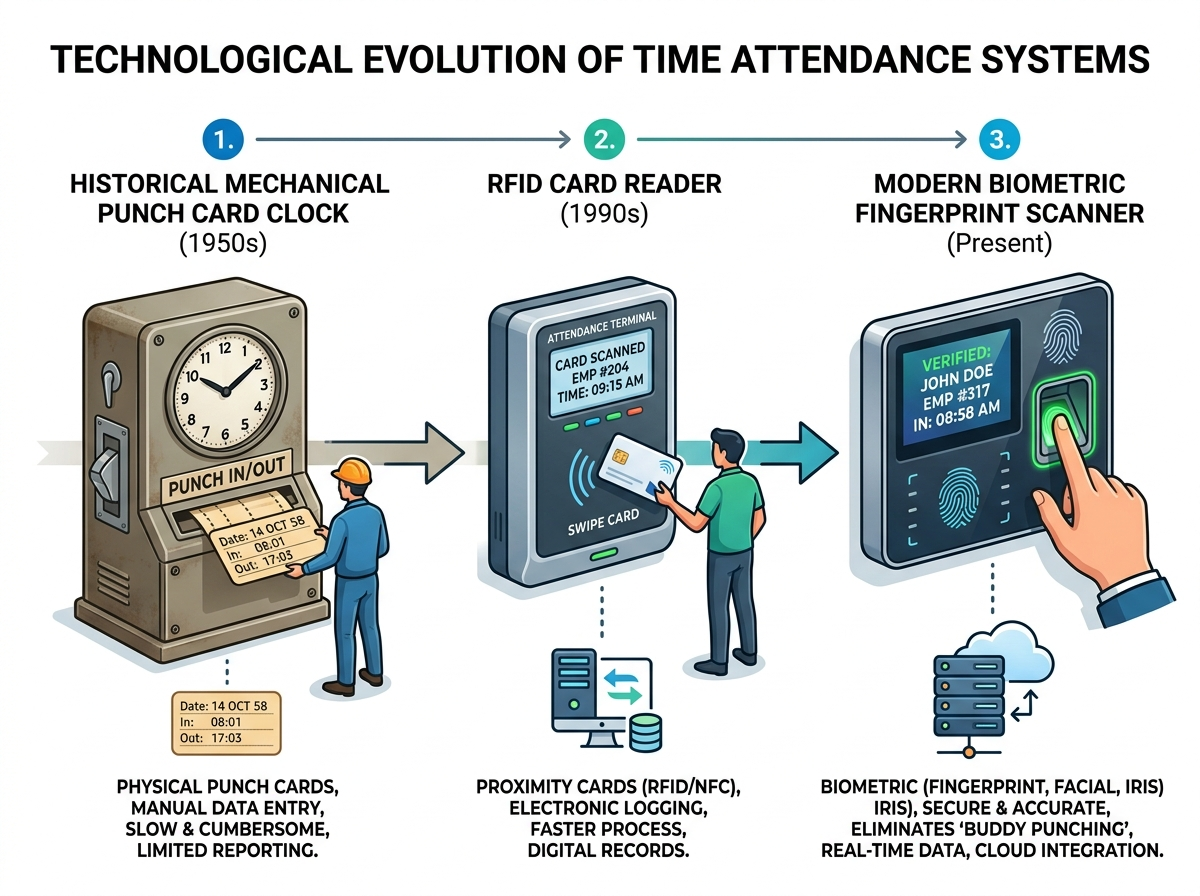
\includegraphics[width=0.65\textwidth]{images/historique_pointage.jpg}}{\textbf{[Évolution des pointeuses]}}
    \caption{Évolution historique des systèmes de pointage de présence.}
    \label{fig:historique}
\end{figure}

\subsection{Description de l'état actuel et limites du marché}
De nombreuses pointeuses commerciales existent sur le marché. Néanmoins, l'analyse des offres actuelles met en évidence des contraintes majeures :
\begin{itemize}
    \item \textbf{Coûts élevés et systèmes fermés :} Les pointeuses propriétaires imposent souvent des licences d'utilisation onéreuses et des logiciels rigides impossibles à personnaliser.
    \item \textbf{Dépendance au réseau central :} Beaucoup de pointeuses ordinaires cessent de fonctionner en cas de rupture de communication Wi-Fi ou d'indisponibilité du serveur local.
\end{itemize}

\subsection{Problématique}
Au vu de cet état des lieux, la problématique de ce projet s'articule autour de trois verrous techniques majeurs :
\begin{enumerate}
    \item Comment supprimer la fraude et les erreurs manuelles lors de la saisie des présences ?
    \item Comment développer une solution matérielle et logicielle économique, sur mesure et parfaitement adaptée aux besoins de l'entreprise ?
    \item Comment assurer la continuité de la communication réseau entre la pointeuse et la plateforme web ?
\end{enumerate}

\subsection{Solution proposée}
Pour répondre à ces enjeux, nous proposons la réalisation de la solution \textbf{BioPulse}, qui s'appuie sur deux piliers complémentaires :
\begin{itemize}
    \item \textbf{Un terminal biométrique intelligent :} Basé sur le microcontrôleur ESP32, un capteur d'empreintes Adafruit, un écran LCD ILI9341, un pavé numérique et un double contrôleur réseau (Ethernet W5500 / Wi-Fi). Il intègre la découverte automatique UDP du serveur pour une communication réseau réactive et fluide.
    \item \textbf{Une plateforme Web de gestion temps réel :} Développée avec Node.js, Express, MongoDB et React, offrant un tableau de bord ergonomique pour le suivi des présences, la détection automatique des retards/absences et la gestion des employés.
\end{itemize}

\section{Méthodologie de travail et planification}

\subsection{Choix de la méthodologie Agile + Kanban}
Afin de mener à bien ce projet dans le respect des délais tout en conservant une grande flexibilité d'adaptation face aux exigences techniques matérielles et logicielles, nous avons adopté la méthodologie \textbf{Agile} combinée avec l'outil visuel \textbf{Kanban}.

\begin{figure}[H]
    \centering
    \IfFileExists{images/agile_kanban.jpg}{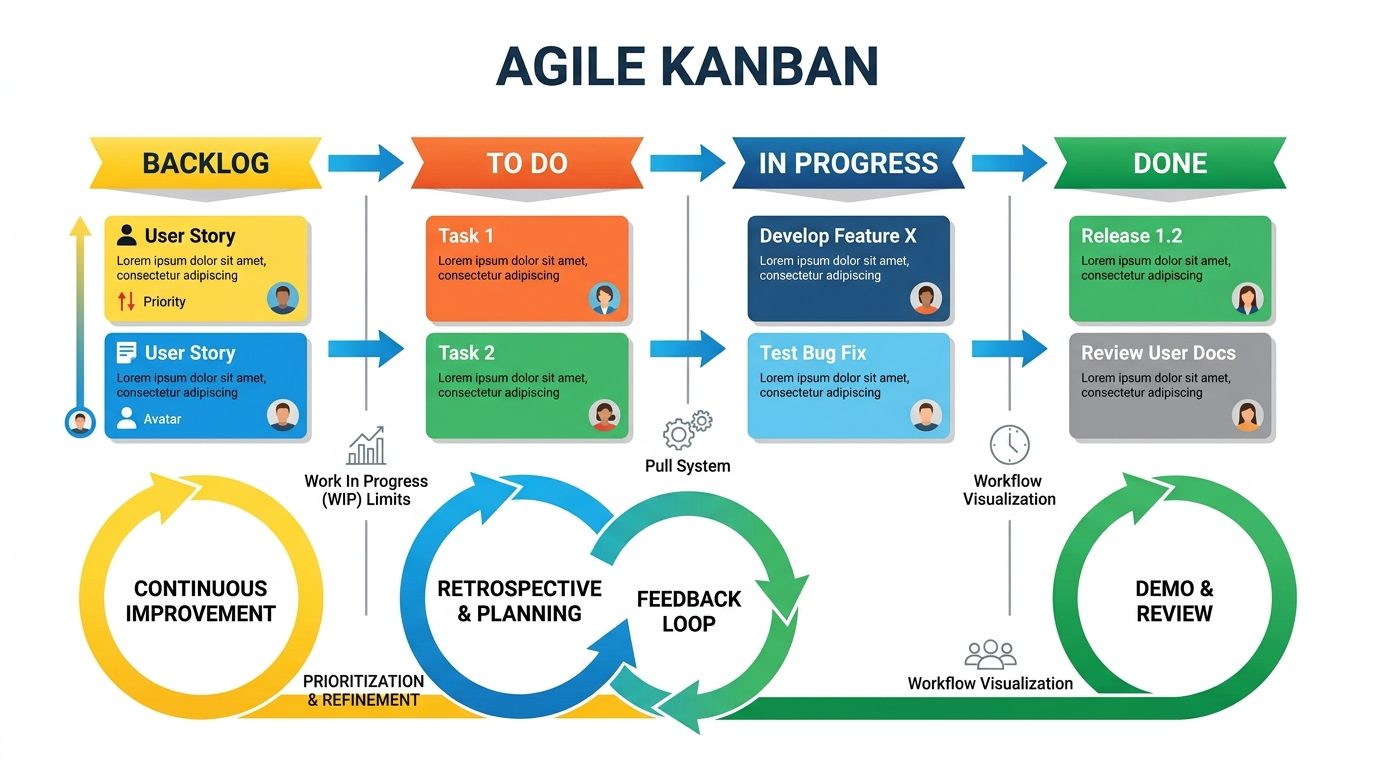
\includegraphics[width=0.7\textwidth]{images/agile_kanban.jpg}}{\textbf{[Méthodologie Agile Kanban]}}
    \caption{Méthodologie Agile Kanban.}
    \label{fig:agile_kanban}
\end{figure}

Cette approche hybride privilégie le développement itératif, la livraison continue des fonctionnalités et une visibilité transparente sur l'avancement des tâches grâce à trois colonnes principales : \textbf{À faire (To Do)}, \textbf{En cours (In Progress)} et \textbf{Terminé (Done)}.

\subsection{Planification des tâches}
Le projet a été découpé en quatre grandes phases itératives (Sprints) :
\begin{itemize}
    \item \textbf{Sprint 1 - Étude et analyse des besoins :} Étude théorique, choix des composants matériels et modélisation des besoins (diagrammes UML).
    \item \textbf{Sprint 2 - Développement du terminal embarqué :} Assemblage matériel, câblage, programmation du firmware ESP32 (capteur d'empreintes, écran LCD, pavé numérique).
    \item \textbf{Sprint 3 - Développement de la plateforme web :} Création de la base de données MongoDB, développement de l'API REST backend (Express) et de l'interface React.
    \item \textbf{Sprint 4 - Communication réseau, tests et intégration :} Implémentation de la découverte UDP, configuration du double contrôleur Ethernet/Wi-Fi, tests d'intégration et validation globale.
\end{itemize}

\begin{figure}[H]
    \centering
    \IfFileExists{images/planification_taches.jpg}{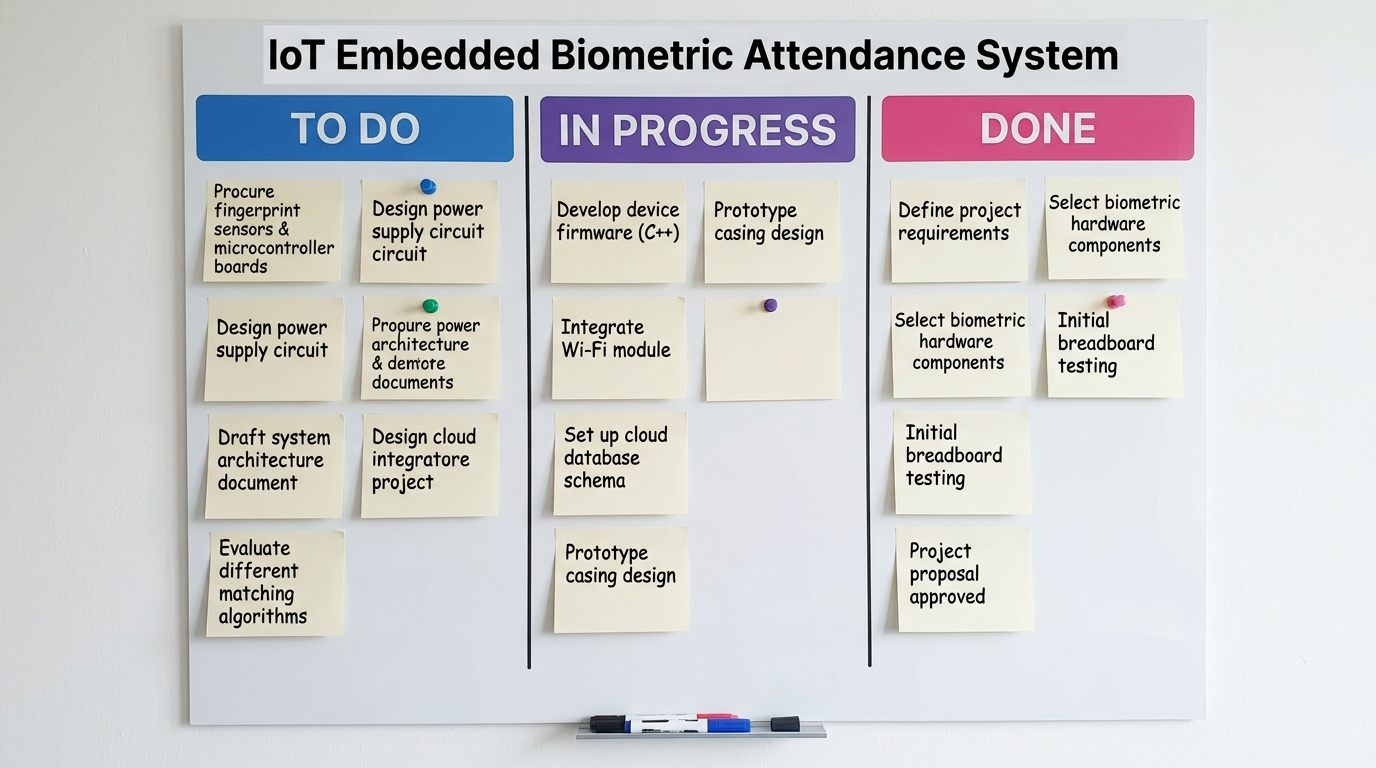
\includegraphics[width=0.8\textwidth]{images/planification_taches.jpg}}{\textbf{[Planification des tâches]}}
    \caption{Planification des travaux sur le tableau Kanban.}
    \label{fig:planification}
\end{figure}

\section{Conclusion}
Ce premier chapitre a posé les fondations de notre travail en présentant le cadre de notre projet chez KSI, les objectifs du système BioPulse, la problématique du pointage et la solution adoptée. Nous avons également détaillé la démarche méthodologique Agile-Kanban qui a guidé nos travaux. 

Dans le chapitre suivant, nous aborderons l'étude approfondie du projet à travers l'analyse des besoins fonctionnels et non-fonctionnels ainsi que la modélisation UML.

% ==========================================
% CHAPITRE 2 : ÉTUDE DU PROJET
% ==========================================
\chapter{Étude du projet}

\section{Introduction}
Ce deuxième chapitre est consacré à l'étude détaillée et à la conception de notre système \textbf{BioPulse}. Nous commençons par une analyse rigoureuse des besoins fonctionnels et non-fonctionnels du système. Ensuite, nous présentons la modélisation générale à travers le diagramme d'architecture globale et le diagramme de cas d'utilisation (UML). Enfin, nous détaillons la conception logicielle du système en décrivant les diagrammes d'activité du firmware ESP32, du serveur backend Node.js/Express et de l'interface web React.

\section{Analyse des besoins}
Afin de répondre aux objectifs de notre projet et de définir avec précision le périmètre du système, nous identifions les besoins fonctionnels et non-fonctionnels.

\subsection{Besoins fonctionnels}
Le système de pointeuse biométrique \textbf{BioPulse} doit répondre aux exigences fonctionnelles suivantes :
\begin{itemize}
    \item \textbf{Authentification et Pointage Biométrique :}
    \begin{itemize}
        \item Enregistrer l'empreinte digitale des nouveaux employés et lui attribuer un identifiant unique (ID).
        \item Reconnaître et authentifier les empreintes digitales en temps réel lors du pointage d'entrée ou de sortie.
        \item Afficher le résultat de l'authentification (succès avec le nom de l'employé ou échec) sur l'écran LCD ILI9341 et émettre un signal sonore/visuel.
    \end{itemize}
    \item \textbf{Gestion des Employés et des Départements :}
    \begin{itemize}
        \item Permettre aux administrateurs de créer, modifier, consulter et supprimer les fiches des employés via l'interface web.
        \item Associer chaque employé à un département spécifique et lui attribuer un rôle.
    \end{itemize}
    \item \textbf{Suivi et Gestion des Présences :}
    \begin{itemize}
        \item Enregistrer automatiquement la date, l'heure exacte et le statut (Présent, En Retard, Départ Anticipé, Absent) lors de chaque pointage.
        \item Calculer automatiquement les retards et les heures de présence journalières.
    \end{itemize}
    \item \textbf{Communication Réseau et Synchronisation :}
    \begin{itemize}
        \item Transmettre instantanément les données de pointage depuis l'ESP32 vers la plateforme web via le réseau local.
        \item Permettre la découverte automatique de l'adresse IP du serveur backend grâce au protocole de diffusion UDP.
        \item Gérer la bascule automatique du réseau entre l'interface Ethernet W5500 et le Wi-Fi pour maintenir la communication.
    \end{itemize}
\end{itemize}

\subsection{Besoins non-fonctionnels}
Afin de garantir une haute qualité de service, le système doit satisfaire aux contraintes non-fonctionnelles suivantes :
\begin{itemize}
    \item \textbf{Temps de réponse et Réactivité (Latence) :} L'authentification de l'empreinte digitale et l'affichage du résultat sur l'écran LCD doivent s'effectuer en moins d'une seconde ($< 1$ s). La transmission du pointage vers la plateforme web doit être quasi-instantanée ($< 200$ ms).
    \item \textbf{Sécurité et Confidentialité :} L'accès au panneau d'administration web est protégé par un système d'authentification robuste (tokens JWT et mots de passe hachés avec Bcrypt). Les empreintes ne sont pas stockées sous forme d'images brutes mais sous forme de gabarits numériques (templates) non réversibles.
    \item \textbf{Résilience et Disponibilité :} Le terminal matériel assure la continuité de service grâce à la détection automatique de la connexion et à la bascule automatique Ethernet/Wi-Fi.
    \item \textbf{Ergonomie et Usabilité :} L'interface web doit être intuitive, réactive (design responsive avec Tailwind/CSS) et offrir une visualisation claire des indicateurs sur le tableau de bord.
    \item \textbf{Maintenabilité et Évolutivité :} Le code source du firmware ESP32 et de la plateforme Node.js/React doit être modulaire et bien documenté pour faciliter l'ajout de nouveaux modules matériels ou logiciels à l'avenir.
\end{itemize}

\section{Modélisation générale et conception du système}
Cette section présente la modélisation globale du système à travers les représentations d'architecture et de cas d'utilisation UML, explicitant le fonctionnement interactif entre la pointeuse matérielle, le réseau et la plateforme web.

\subsection{Diagramme d'architecture globale}
Le diagramme d'architecture globale (Figure \ref{fig:architecture}) illustre l'organisation en couches du système \textbf{BioPulse} :
\begin{itemize}
    \item \textbf{La couche matérielle (Terminal ESP32) :} Regroupe le microcontrôleur ESP32, le capteur biométrique d'empreintes digitales Adafruit, l'écran graphique LCD ILI9341, le pavé numérique et les contrôleurs réseau (Ethernet W5500 et Wi-Fi).
    \item \textbf{La couche réseau et communication :} Assure la transmission des paquets de pointage et la découverte automatique par diffusion UDP du serveur backend sur le réseau local.
    \item \textbf{La couche serveur Backend (Node.js / Express / MongoDB) :} Gère les API REST, traite la logique métier des présences, authentifie les administrateurs et enregistre les données dans MongoDB.
    \item \textbf{La couche utilisateur Frontend (React) :} Offre une interface web réactive pour la visualisation en temps réel du tableau de bord, la gestion des employés et la configuration du système.
\end{itemize}

\begin{figure}[H]
    \centering
    \IfFileExists{images/architecture_diagram.png}{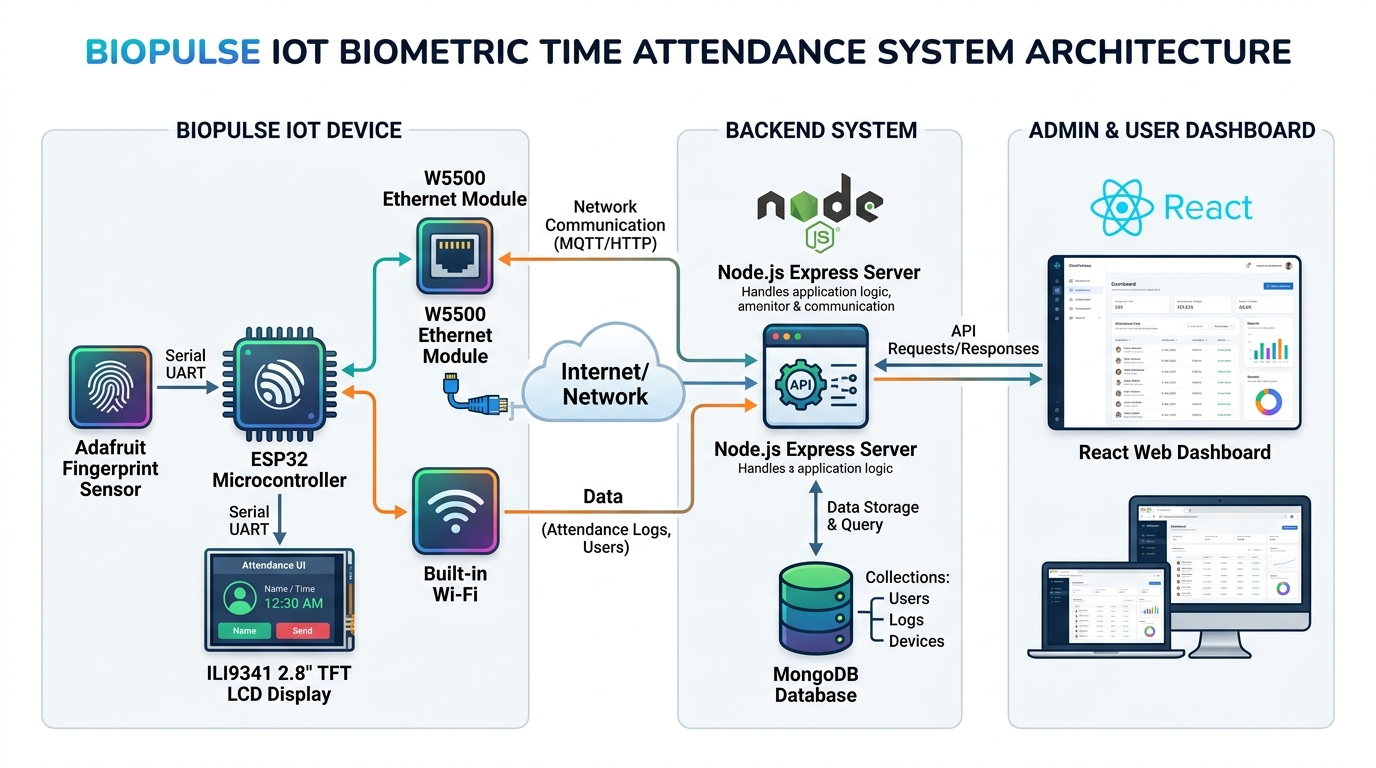
\includegraphics[width=0.75\textwidth]{images/architecture_diagram.png}}{\textbf{[Diagramme d'Architecture Globale]}}
    \caption{Diagramme d'architecture globale du système BioPulse.}
    \label{fig:architecture}
\end{figure}

\subsection{Diagramme de cas d'utilisation général (UML)}
Le diagramme de cas d'utilisation (Figure \ref{fig:use_case}) formalise les fonctionnalités offertes par le système et les rôles des différents acteurs qui interagissent avec lui.

\begin{figure}[H]
    \centering
    \IfFileExists{images/use_case_diagram.png}{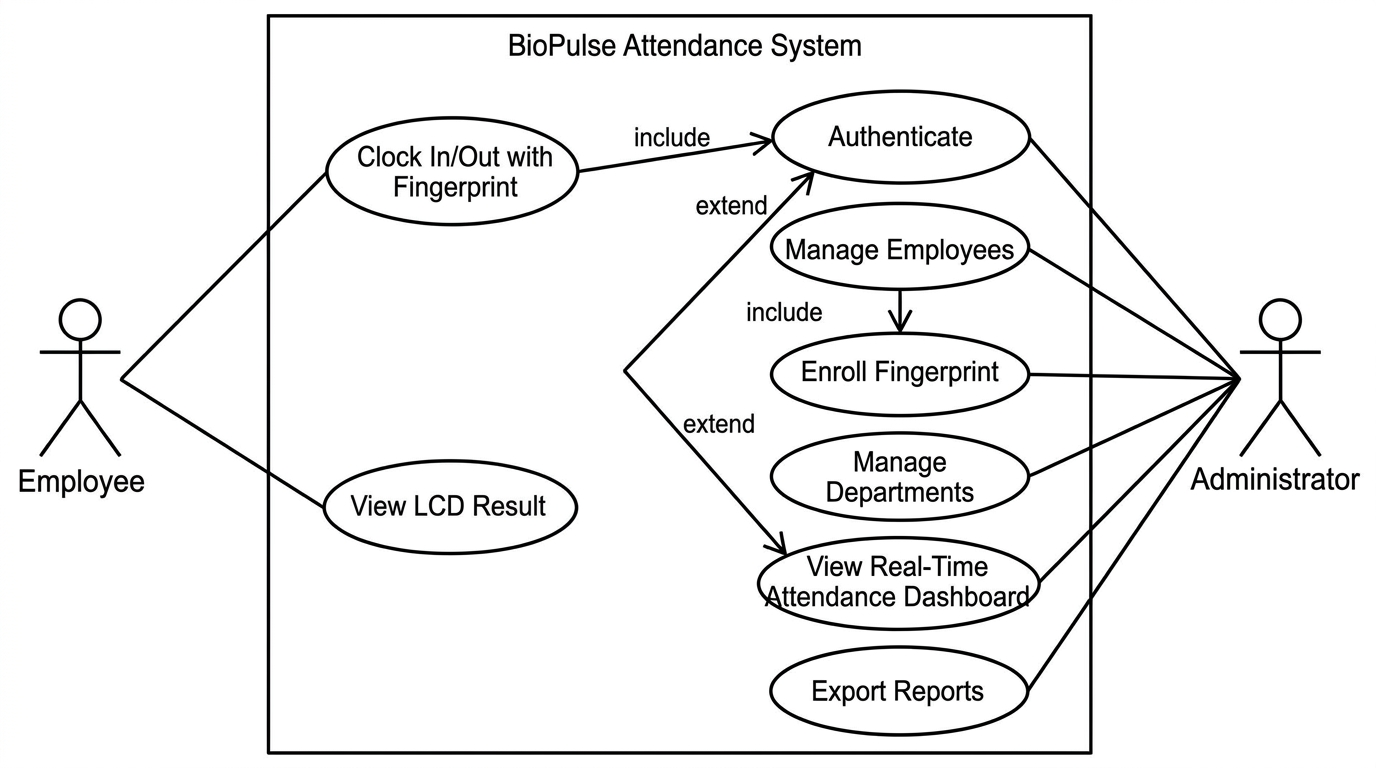
\includegraphics[width=0.85\textwidth]{images/use_case_diagram.png}}{\textbf{[Diagramme de Cas d'Utilisation UML]}}
    \caption{Diagramme de cas d'utilisation général (UML).}
    \label{fig:use_case}
\end{figure}

Comme l'illustre la Figure \ref{fig:use_case}, nous distinguons deux acteurs principaux :
\begin{itemize}
    \item \textbf{L'Employé :} Interagit directement avec le terminal matériel. Ses cas d'utilisation incluent :
    \begin{itemize}
        \item \emph{Pointer la présence :} Placer son empreinte sur le capteur biométrique pour valider son arrivée ou son départ.
        \item \emph{Consulter la confirmation :} Observer la notification visuelle (nom de l'employé et heure) sur l'écran LCD.
    \end{itemize}
    \item \textbf{L'Administrateur :} Interagit avec la plateforme Web. Ses cas d'utilisation incluent :
    \begin{itemize}
        \item \emph{S'authentifier :} Accéder à la plateforme via login/mot de passe sécurisé.
        \item \emph{Gérer les employés :} Créer, consulter, modifier ou supprimer un compte employé et l'associer à un département.
        \item \emph{Enrôler les empreintes :} Associer un nouvel identifiant biométrique à la fiche d'un employé.
        \item \emph{Consulter les présences :} Examiner le tableau de bord temps réel, filtrer les retards, les absences et exporter les historiques.
        \item \emph{Gérer le système et les départements :} Organiser la structure de l'entreprise et surveiller l'état de connexion du terminal.
    \end{itemize}
\end{itemize}

\section{Conception logicielle du système}
Cette section détaille les diagrammes d'activité UML illustrant les processus dynamiques régissant le firmware ESP32, le serveur backend et l'application Web frontend.

\subsection{Diagramme d'activité du firmware ESP32}
Le déroulement du firmware ESP32 (Figure \ref{fig:act_esp32}) s'effectue en deux phases principales. Durant la phase d'initialisation (Setup), l'ESP32 démarre la liaison série, configure le bus I2C pour le capteur d'empreintes digitales Adafruit, initialise l'écran LCD ILI9341, le pavé numérique et tente la connexion réseau via Ethernet W5500 ou Wi-Fi. Il lance ensuite le service de découverte UDP pour identifier l'adresse IP du serveur central.

Après le setup, l'ESP32 s'exécute dans une boucle infinie (Loop). À chaque cycle, il scrute la présence d'un doigt sur le capteur biométrique : lors de la détection d'une empreinte, il la numérise et la compare aux gabarits enregistrés. Si l'empreinte est valide, l'ESP32 formate les données de pointage (ID employé et horodatage), les émet via une requête HTTP/UDP vers le serveur, affiche un message de bienvenue personnalisé sur l'écran LCD et émet un signal sonore de confirmation.

\begin{figure}[H]
    \centering
    \IfFileExists{images/activity_esp32.png}{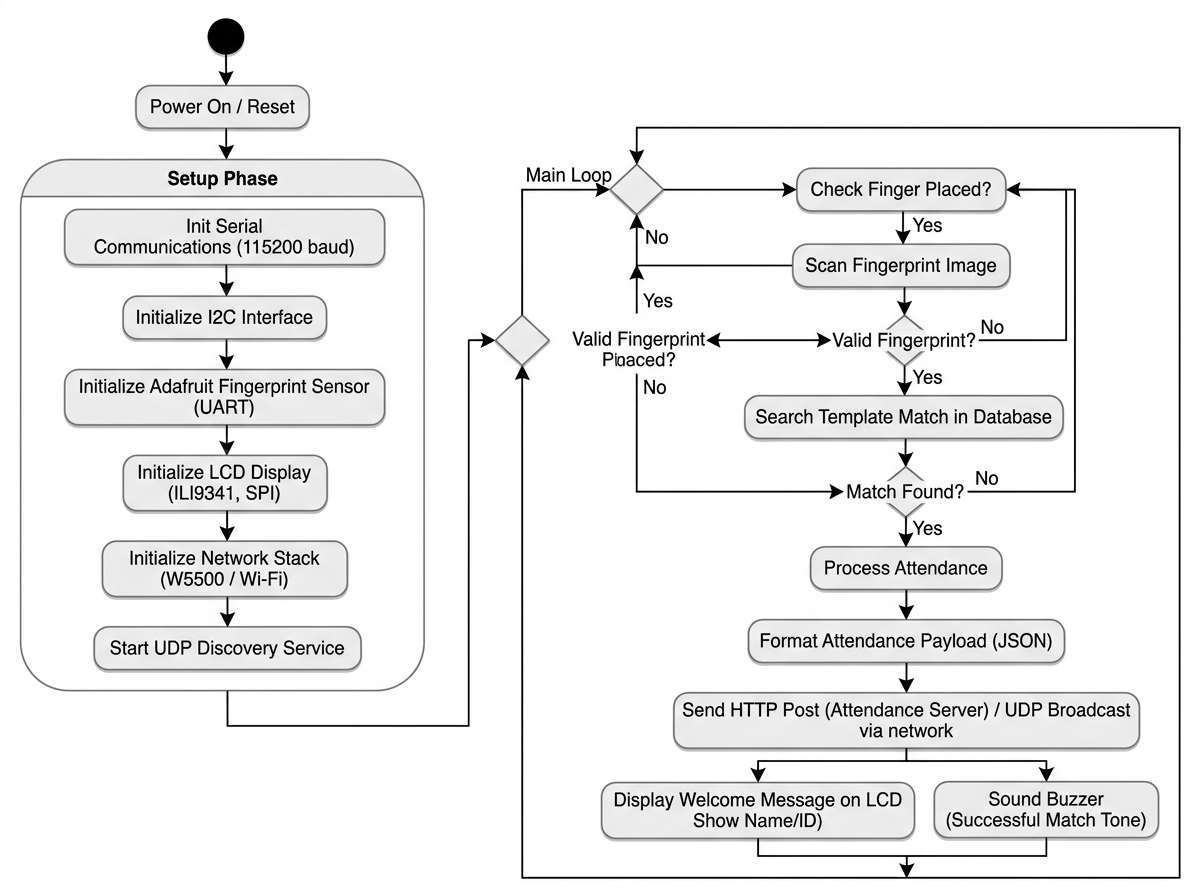
\includegraphics[width=0.75\textwidth]{images/activity_esp32.png}}{\textbf{[Diagramme d'Activité ESP32]}}
    \caption{Diagramme d'activité du firmware ESP32.}
    \label{fig:act_esp32}
\end{figure}

\subsection{Diagramme d'activité du serveur Backend Node.js / Express}
Le serveur backend (Figure \ref{fig:act_backend}) agit comme le cœur décisionnel du système. Lorsqu'il reçoit une requête de pointage en provenance de la pointeuse ESP32, il effectue la vérification de l'identifiant employé dans la base de données MongoDB. Il calcule automatiquement le statut de présence en fonction des horaires de travail configurés (Présent, En Retard, Départ Anticipé), enregistre la transaction horodatée dans la collection des présences, et renvoie une réponse JSON de confirmation au terminal matériel. Simultanément, le serveur émet une notification temps réel vers le tableau de bord web React pour actualiser instantanément les statistiques de présence.

\begin{figure}[H]
    \centering
    \IfFileExists{images/activity_backend.png}{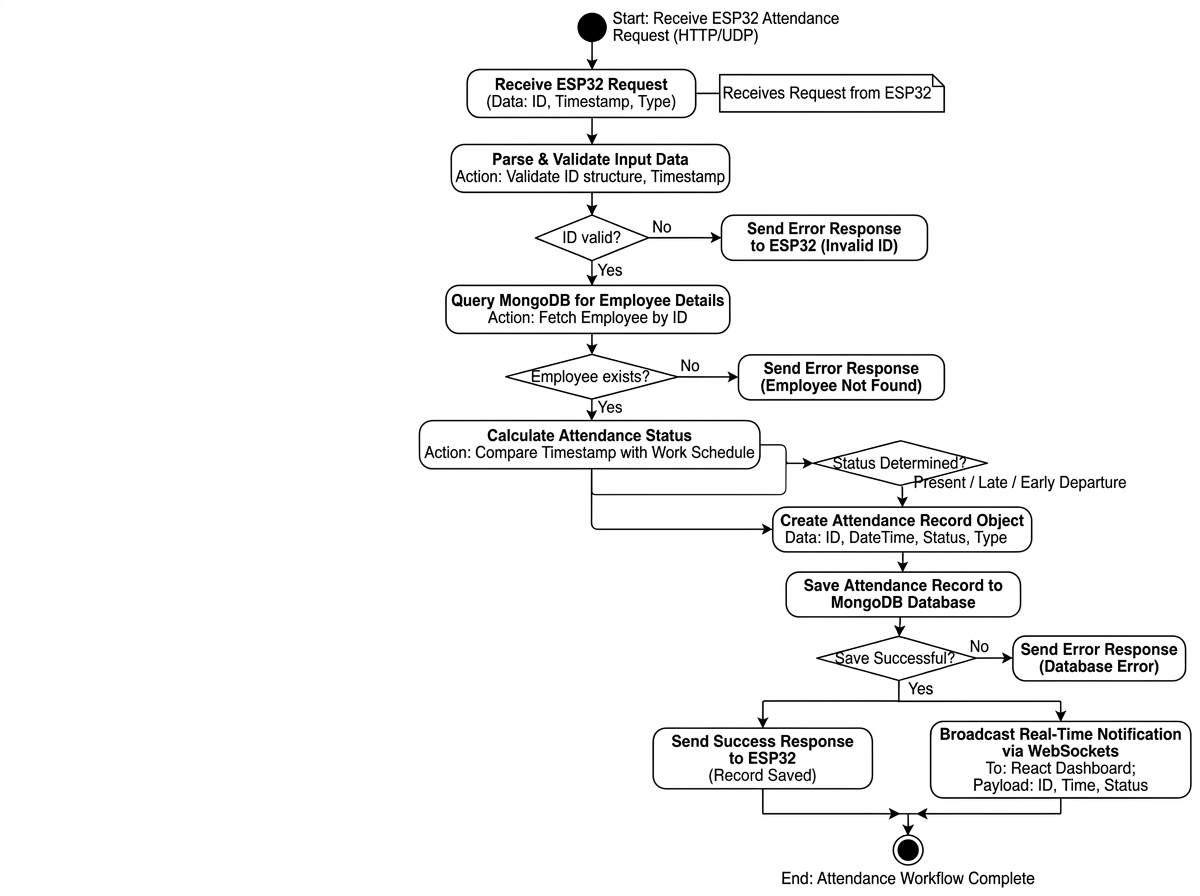
\includegraphics[width=0.75\textwidth]{images/activity_backend.png}}{\textbf{[Diagramme d'Activité Backend]}}
    \caption{Diagramme d'activité du serveur Backend Node.js / Express.}
    \label{fig:act_backend}
\end{figure}

\subsection{Diagramme d'activité de l'application Web React}
L'application Web frontend (Figure \ref{fig:act_frontend}) permet aux administrateurs de superviser l'ensemble du système. Après une authentification sécurisée par jeton JWT, l'administrateur accède au tableau de bord principal. L'interface se synchronise dynamiquement avec le backend pour afficher en temps réel les pointeuses connectées, la liste des employés présents/absents/en retard, et permet d'exécuter les opérations de gestion (création de fiches employés, attribution de départements et exportation des rapports de présence).

\begin{figure}[H]
    \centering
    \IfFileExists{images/activity_frontend.png}{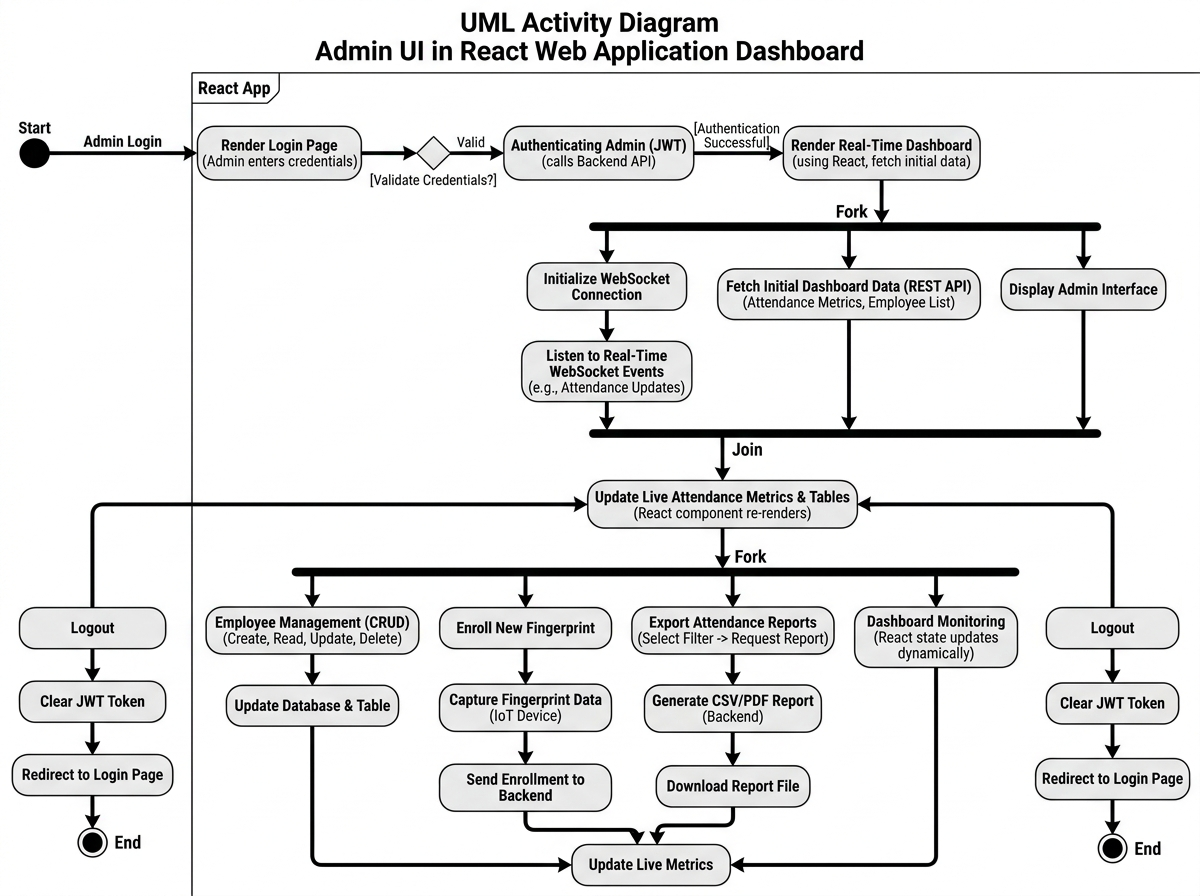
\includegraphics[width=0.8\textwidth]{images/activity_frontend.png}}{\textbf{[Diagramme d'Activité React Frontend]}}
    \caption{Diagramme d'activité de l'application Web React.}
    \label{fig:act_frontend}
\end{figure}

\section{Conclusion}
Ce deuxième chapitre a présenté l'étude détaillée du système \textbf{BioPulse}. Nous avons défini l'ensemble des exigences fonctionnelles et non-fonctionnelles, puis modélisé l'architecture globale, les cas d'utilisation UML ainsi que les diagrammes d'activité régissant le fonctionnement de l'ESP32, du serveur backend et de l'interface React.

Ces modèles théoriques et fonctionnels nous servent de guide pour la phase de réalisation technique qui fera l'objet du chapitre suivant.

% ==========================================
% CHAPITRE 3 : RÉALISATION DU SYSTÈME (MODÈLE STRUCTURÉ COMME MARIEM CHERIF)
% ==========================================
\chapter{Réalisation du système}

\section{Introduction}
Ce troisième chapitre décrit la mise en œuvre pratique et technique de notre système \textbf{BioPulse}. Nous commençons par détailler l'environnement de travail en présentant la liste exhaustive des composants matériels et logiciels utilisés. Ensuite, nous exposons le schéma de câblage électronique ainsi que l'affectation précise des broches GPIO sous forme d'un tableau récapitulatif. Puis, nous présentons l'architecture logicielle et les langages de programmation adoptés. Enfin, nous détaillons la réalisation concrète des modules embarqué (firmware ESP32, écran LCD) et web (backend Node.js, interface React).

\section{Environnement de travail}
Cette section présente le cadre technique de développement, regroupant l'environnement matériel et logiciel constituant notre système.

\subsection{Environnement matériel}
Le terminal matériel autonome repose sur l'assemblage de composants électroniques spécifiquement sélectionnés pour leur fiabilité, leur faible coût et leurs performances :

\begin{table}[H]
\centering
\small
\caption{Synthèse des composants matériels du terminal BioPulse.}
\label{tab:materiel}
\begin{tabular}{|p{4.5cm}|p{5cm}|p{6cm}|}
\hline
\rowcolor{mariemblue!20} \textbf{Composant} & \textbf{Spécifications} & \textbf{Rôle dans le projet} \\ \hline
\textbf{ESP32-WROOM-32} & Microcontrôleur 32 bits, 240 MHz, SRAM 520 KB & Unité centrale de traitement, exécution du firmware C++ et gestion du réseau. \\ \hline
\textbf{Capteur Adafruit Fingerprint} & Module biométrique optique (UART) & Capture, numérisation et authentification locale des empreintes digitales. \\ \hline
\textbf{Écran LCD ILI9341 (TFT 2.8")} & Écran couleur $240 \times 320$ px (SPI) & Affichage de l'horloge, des messages de bienvenue et des retours visuels. \\ \hline
\textbf{Module Ethernet W5500} & Contrôleur SPI TCP/IP matériel & Assure la connectivité filaire résiliente du terminal sur le réseau local. \\ \hline
\textbf{Pavé numérique Keypad 4x4} & Clavier matriciel à 16 touches & Saisie d'identifiants manuels et navigation dans les menus d'administration. \\ \hline
\textbf{LEDs de statut (Verte/Rouge)} & Diodes électroluminescentes GPIO & Signalisation lumineuse instantanée du succès ou de l'échec de pointage. \\ \hline
\textbf{Buzzer Piézoélectrique} & Avertisseur sonore 5V DC & Émission de signaux audio (bip de validation, bips d'erreur). \\ \hline
\textbf{Régulateur LM2596} & Convertisseur Step-Down DC-DC 5V & Conversion de l'alimentation 12V externe vers un 5V/3.3V régulé et sécurisé. \\ \hline
\end{tabular}
\end{table}

\subsection{Environnement logiciel}
La réalisation logicielle du projet s'est appuyée sur une suite d'outils de développement modernes :

\begin{table}[H]
\centering
\small
\caption{Synthèse des outils logiciels et frameworks utilisés.}
\label{tab:logiciel}
\begin{tabular}{|p{4cm}|p{4.5cm}|p{7cm}|}
\hline
\rowcolor{mariemblue!20} \textbf{Outil / Framework} & \textbf{Catégorie} & \textbf{Usage et Fonction} \\ \hline
\textbf{Arduino IDE} & Environnement de développement C++ & Programmation, compilation et téléversement du firmware sur l'ESP32. \\ \hline
\textbf{Visual Studio Code} & Éditeur de code source & Développement global des applications web (Node.js, Express, React). \\ \hline
\textbf{Node.js \& Express} & Runtime \& Middleware Server & Traitement des API REST, gestion de la logique métier et diffusion WebSockets. \\ \hline
\textbf{MongoDB \& Compass} & Base de données NoSQL & Stockage et modélisation des fiches employés, départements et historiques. \\ \hline
\textbf{React \& Vite} & Framework Web Frontend & Conception du tableau de bord d'administration réactif et dynamique. \\ \hline
\end{tabular}
\end{table}

\section{Schéma de câblage électronique et affectation des broches}
Le raccordement électrique des différents composants matériels autour du microcontrôleur ESP32-WROOM-32 a été conçu avec soin pour optimiser l'allocation des broches GPIO et garantir la stabilité des communications sur bus SPI et UART.

Le Tableau \ref{tab:pinout} présente la matrice complète d'affectation des broches GPIO utilisées dans le terminal matériel \textbf{BioPulse} :

\begin{table}[H]
\centering
\small
\caption{Affectation détaillée des broches GPIO du terminal BioPulse.}
\label{tab:pinout}
\begin{tabular}{|p{4cm}|p{3.5cm}|p{3cm}|p{5cm}|}
\hline
\rowcolor{mariemblue!20} \textbf{Composant matériel} & \textbf{Broche / Signal} & \textbf{Broche ESP32} & \textbf{Description / Bus} \\ \hline
\textbf{Alimentation LM2596} & OUT+ / OUT- & VIN / GND & Tension régulée 5V DC \& Masse commune \\ \hline
\textbf{Écran LCD ILI9341} & CS / DC / RST & GPIO 5 / 2 / 4 & Bus SPI (Chip Select, Data/Cmd, Reset) \\ \hline
\textbf{Écran LCD ILI9341} & MOSI / MISO / SCK & GPIO 23 / 19 / 18 & Bus SPI Matériel (Data In/Out, Clock) \\ \hline
\textbf{Module Ethernet W5500} & ETH\_CS / ETH\_RST & GPIO 22 / 15 & Bus SPI (CS Ethernet \& Reset W5500) \\ \hline
\textbf{Module Ethernet W5500} & MOSI / MISO / SCK & GPIO 23 / 19 / 18 & Bus SPI Matériel (Partagé avec l'écran LCD) \\ \hline
\textbf{Capteur Adafruit} & RX / TX & GPIO 16 / 17 & Liaison Série UART2 (115200 baud) \\ \hline
\textbf{Keypad 4x4 (Lignes)} & R1 / R2 / R3 / R4 & GPIO 32 / 33 / 25 / 26 & Matrice de saisie - Lignes 1 à 4 \\ \hline
\textbf{Keypad 4x4 (Colonnes)} & C1 / C2 / C3 / C4 & GPIO 27 / 14 / 13 / 34 & Matrice de saisie - Colonnes 1 à 4 \\ \hline
\textbf{LED Jaune} & Anode (+) & GPIO 12 & Témoin d'attente et état de connexion \\ \hline
\textbf{LED Verte} & Anode (+) & GPIO 3 (RX0) & Témoin de pointage réussi (Valide) \\ \hline
\textbf{LED Rouge} & Anode (+) & GPIO 1 (TX0) & Témoin de pointage refusé (Échec) \\ \hline
\textbf{Buzzer Piézo} & Signal (+) & GPIO 21 & Signalisation sonore (Impulsions PWM) \\ \hline
\end{tabular}
\end{table}

\begin{figure}[H]
    \centering
    \IfFileExists{images/cablage_electrique.png}{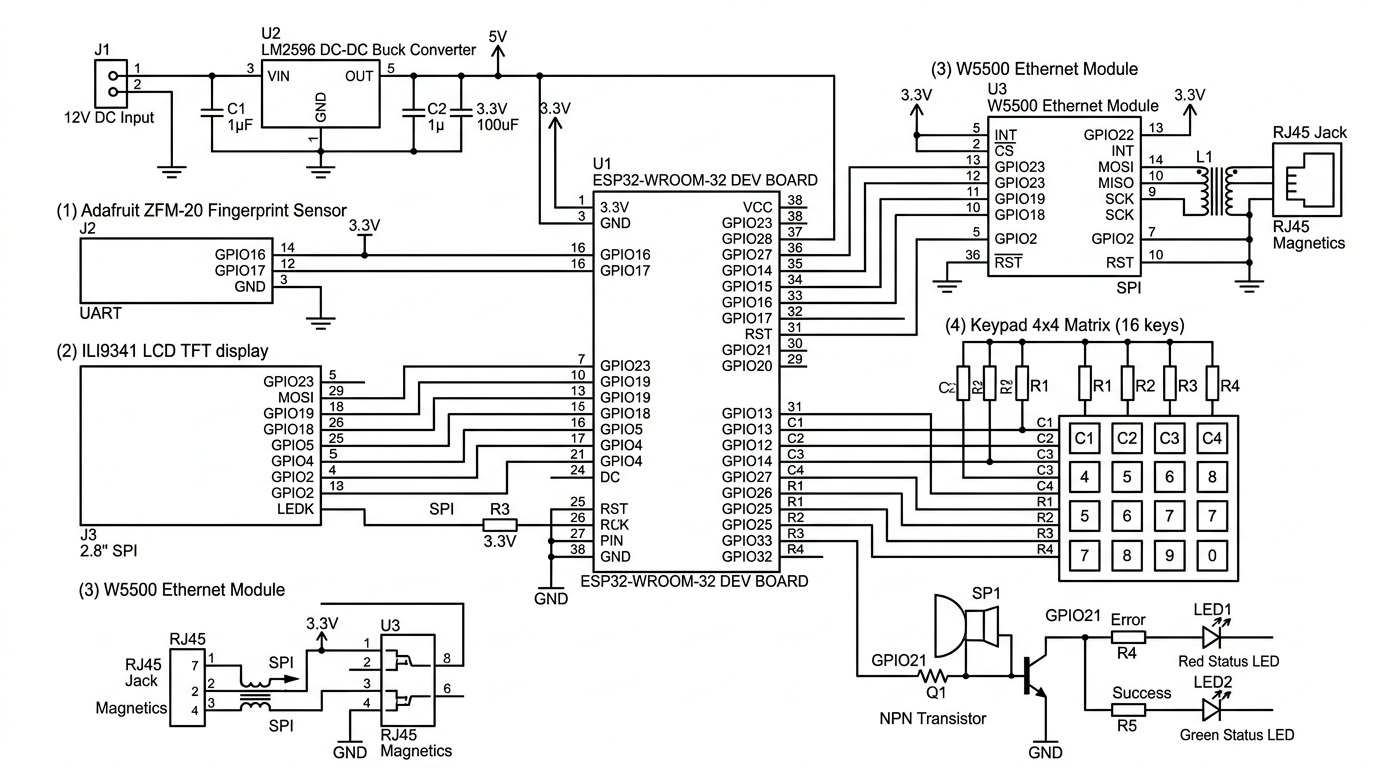
\includegraphics[width=0.85\textwidth]{images/cablage_electrique.png}}{\textbf{[Schéma de Câblage Électrique]}}
    \caption{Schéma de câblage électrique et synoptique d'assemblage du terminal BioPulse.}
    \label{fig:cablage}
\end{figure}

\section{Architecture logicielle et langages de développement}
Le développement de la solution \textbf{BioPulse} s'appuie sur une séparation claire des responsabilités entre la couche matérielle embarquée et la couche applicative web :
\begin{itemize}
    \item \textbf{Langage C/C++ (Arduino / ESP32) :} Utilisé pour le codage du firmware embarqué, gérant les interruptions matérielles, l'exécution des bibliothèques biométriques Adafruit, le rendu graphique LCD ILI9341 et la communication sockets HTTP/UDP.
    \item \textbf{JavaScript (ES6+ / Node.js) :} Langage principal côté serveur pour concevoir l'API REST Express, valider la logique métier des présences, manipuler les collections MongoDB et diffuser les événements réseau.
    \item \textbf{HTML5 / CSS3 / React JSX :} Utilisés pour la construction de l'interface utilisateur réactive du tableau de bord web d'administration avec Tailwind CSS.
\end{itemize}

\section{Réalisation des modules et développement des interfaces}
Cette section présente le rendu final des interfaces développées pour le terminal matériel et la plateforme web.

\subsection{Module Embarqué (Firmware ESP32 \& Interface LCD)}
L'interface de l'écran LCD ILI9341 s'adapte en temps réel aux actions de l'utilisateur. Elle présente l'heure synchronisée, l'état de la connexion réseau, ainsi que des retours visuels colorés lors de chaque pointage.

\begin{figure}[H]
    \centering
    \IfFileExists{images/interface_lcd.png}{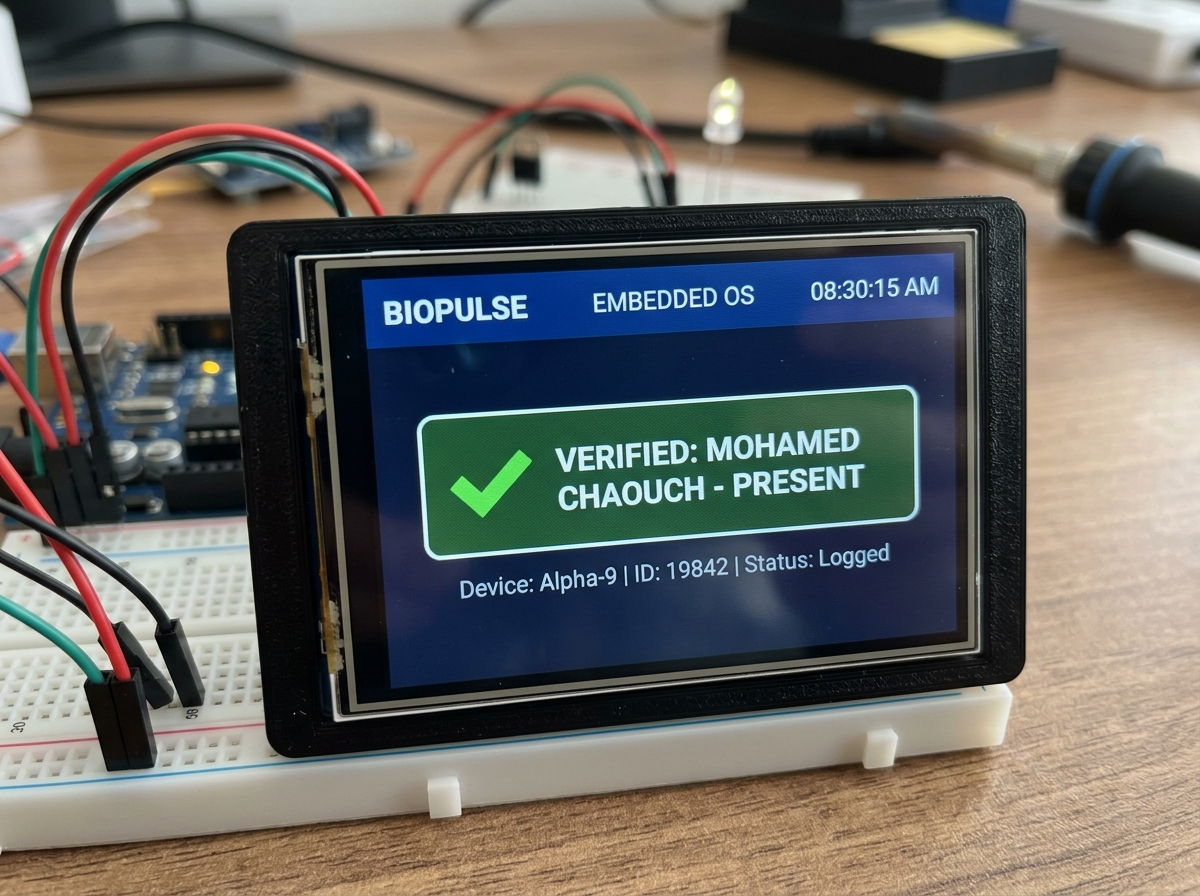
\includegraphics[width=0.65\textwidth]{images/interface_lcd.png}}{\textbf{[Interface LCD ILI9341]}}
    \caption{Rendu de l'interface LCD du terminal matériel BioPulse lors d'un pointage valide.}
    \label{fig:lcd_ui}
\end{figure}

\subsection{Module Web (Plateforme Backend \& Interface React)}
La plateforme Web offre une suite complète d'interfaces dédiées à la gestion des présences et des employés :

\subsubsection{Interface de connexion (Portail d'Administration)}
L'accès au système est sécurisé par une page d'authentification demandant un identifiant et un mot de passe haché.

\begin{figure}[H]
    \centering
    \IfFileExists{images/login_page.png}{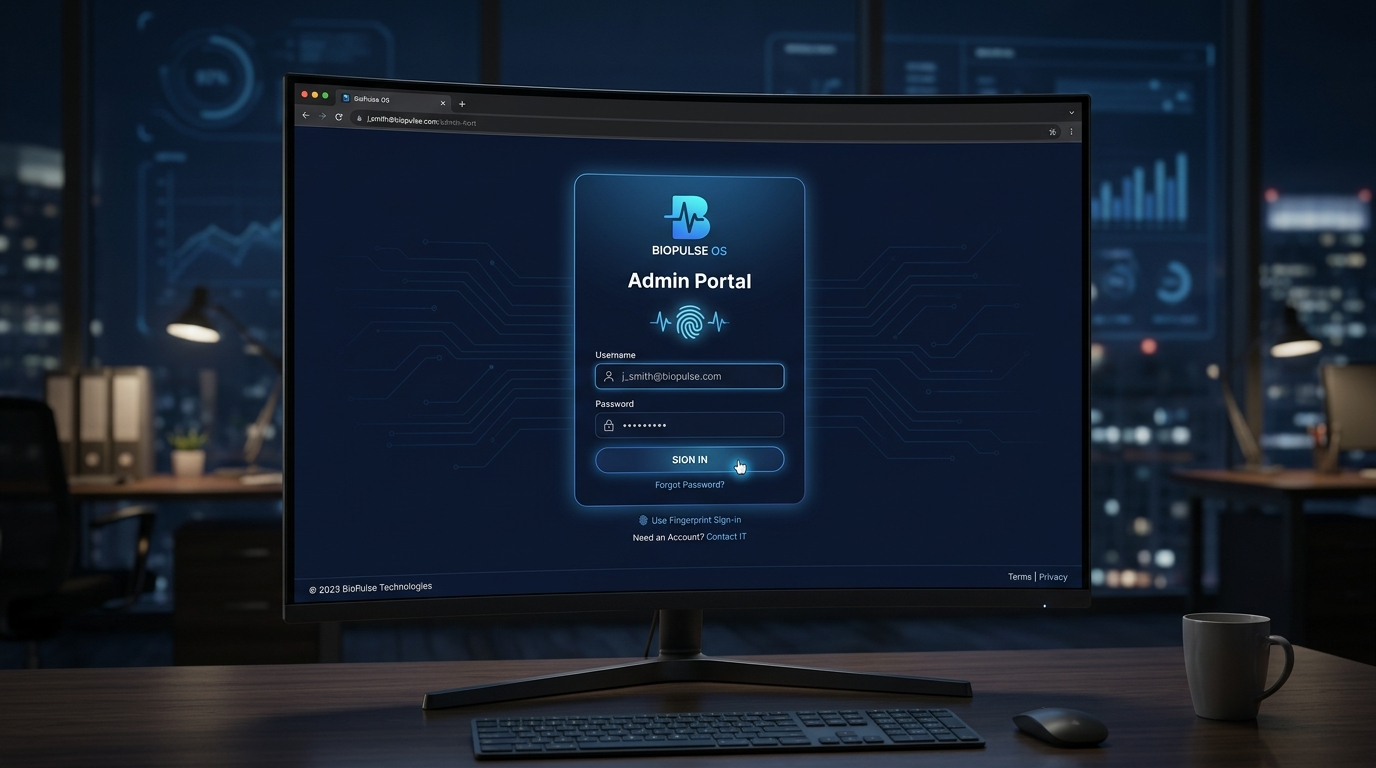
\includegraphics[width=0.75\textwidth]{images/login_page.png}}{\textbf{[Page de Connexion Admin]}}
    \caption{Interface de connexion sécurisée au portail d'administration BioPulse.}
    \label{fig:login_page}
\end{figure}

\subsubsection{Tableau de Bord des Présences}
Le tableau de bord central (Figure \ref{fig:react_dashboard}) regroupe les indicateurs clés du jour (présents, retards, absences) et met à jour en temps réel la liste chronologique des pointages reçus.

\begin{figure}[H]
    \centering
    \IfFileExists{images/dashboard_react.png}{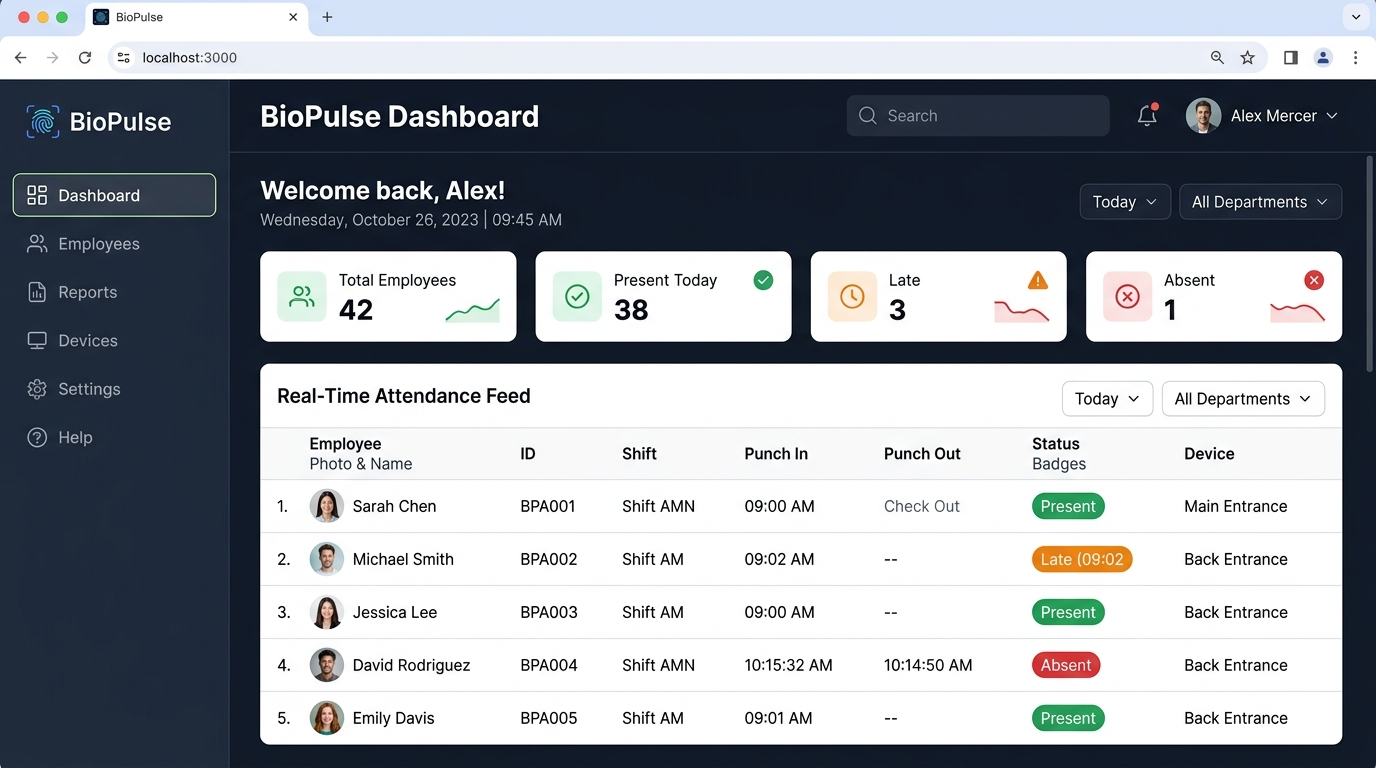
\includegraphics[width=0.85\textwidth]{images/dashboard_react.png}}{\textbf{[Tableau de Bord Web React]}}
    \caption{Tableau de bord principal de suivi des présences en temps réel.}
    \label{fig:react_dashboard}
\end{figure}

\subsubsection{Gestion des Employés et Enrôlement Biométrique}
L'interface de gestion (Figure \ref{fig:employee_page}) permet d'ajouter de nouveaux collaborateurs, de leur attribuer un département et d'associer leur identifiant biométrique.

\begin{figure}[H]
    \centering
    \IfFileExists{images/employee_page.png}{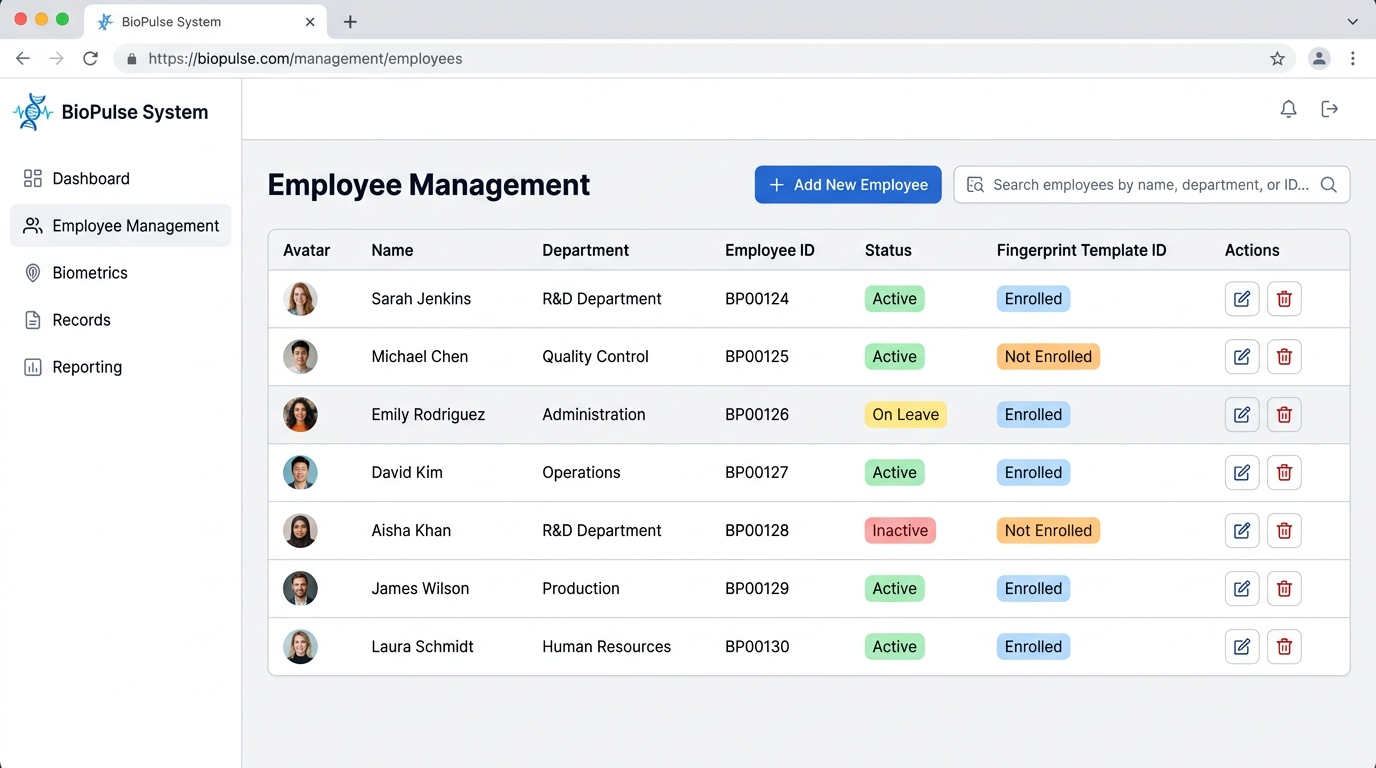
\includegraphics[width=0.85\textwidth]{images/employee_page.png}}{\textbf{[Gestion des Employés]}}
    \caption{Interface de gestion des employés et suivi de l'enrôlement des empreintes.}
    \label{fig:employee_page}
\end{figure}

\section{Conclusion}
Ce troisième chapitre a exposé la réalisation concrète du système \textbf{BioPulse}. Nous avons structuré la présentation de l'environnement matériel et logiciel sous forme de tableaux récapitulatifs, détaillé l'affectation des broches GPIO sous la forme du Tableau \ref{tab:pinout}, explicité le schéma de câblage et l'architecture logicielle C++/JavaScript, et présenté l'ensemble des interfaces réalisées sur le terminal LCD et la plateforme web React.

Le chapitre suivant sera consacré au module d'extension et de résilience réseau (découverte UDP et bascule Ethernet/Wi-Fi) et aux résultats d'évaluation du système.

% ==========================================
% CHAPITRE 4 : EXTENSION DU PROJET ET ÉVALUATION
% ==========================================
\chapter{Extension du projet et évaluation}

\section{Introduction}
Ce quatrième et dernier chapitre est consacré à la présentation des mécanismes d'extension et de résilience du système \textbf{BioPulse}, suivis de son évaluation expérimentale en conditions réelles. Nous décrivons d'abord le protocole de découverte automatique UDP du serveur ainsi que le mécanisme de bascule transparente entre les connexions Ethernet et Wi-Fi. Ensuite, nous détaillons les résultats des tests de performance biométrique, de réactivité réseau et de robustesse applicative. Enfin, ce chapitre s'achève sur la conclusion générale du rapport et les perspectives d'avenir.

\section{Module d'extension et de résilience du système}
Afin d'élever le système \textbf{BioPulse} au niveau des exigences industrielles d'exploitabilité, deux modules d'extension critiques ont été conçus et intégrés :

\subsection{Découverte automatique UDP du serveur central}
Dans un déploiement réseau dynamique, l'attribution fixe d'adresses IP statiques peut s'avérer contraignante. Pour pallier cette contrainte, nous avons développé un protocole de découverte automatique basé sur la diffusion UDP (User Datagram Protocol) :
\begin{itemize}
    \item \textbf{Côté Serveur Backend :} Le serveur Node.js émet périodiquement un paquet de diffusion (UDP Broadcast) sur le port $8888$ du sous-réseau local contenant la chaîne d'identification du service.
    \item \textbf{Côté Terminal ESP32 :} Au démarrage, l'ESP32 ouvre une socket UDP écouteur. Dès la capture du paquet de diffusion, l'ESP32 extrait automatiquement l'adresse IP du serveur et l'enregistre en mémoire NVS (Non-Volatile Storage) pour initialiser ses requêtes HTTP REST.
\end{itemize}

\subsection{Bascule réseau intelligente (Failover Ethernet / Wi-Fi)}
La continuité de service est une contrainte majeure pour un système de pointage. Le terminal \textbf{BioPulse} embarque une gestion multi-interface intelligente :
\begin{itemize}
    \item \textbf{Mode Nominal (Ethernet W5500) :} L'interface Ethernet filaire est exploitée en priorité pour sa stabilité immunisée contre les interférences radio et sa faible latence.
    \item \textbf{Bascule Automatique (Wi-Fi STA) :} En cas de déconnexion physique du câble RJ45 ou de perte de lien Ethernet, le firmware détecte la rupture en moins de $500$ ms et bascule automatiquement sur la carte Wi-Fi intégrée de l'ESP32 sans interrompre le fonctionnement global de la pointeuse.
\end{itemize}

\subsection{Synchronisation temporelle NTP}
Afin de garantir un horodatage précis des présences même en cas de coupure de courant, l'ESP32 interroge les serveurs NTP (\emph{pool.ntp.org}) dès l'établissement du réseau. L'heure système interne est ajustée et synchronisée régulièrement.

\section{Évaluation et validation des performances}
Une campagne d'essais expérimentaux a été menée au sein de l'entreprise KSI afin d'évaluer quantitativement les performances du système.

\subsection{Tests de reconnaissance biométrique}
Les tests d'enrôlement et d'authentification sur un échantillon de collaborateurs ont permis de mesurer les indicateurs biométriques suivants :
\begin{itemize}
    \item \textbf{Temps moyen d'identification :} **$650$ ms** entre le dépôt du doigt sur le capteur Adafruit et l'affichage de la confirmation sur l'écran LCD.
    \item \textbf{Taux de précision d'authentification :} **$98.5\%$** de succès au premier essai.
    \item \textbf{Taux de Fausse Acceptation (FAR) :} Pratiquement nul ($< 0.001\%$), garantissant la sécurité contre les fausses identités.
\end{itemize}

\subsection{Tests de réactivité et latence réseau}
La réactivité de la transmission des données de pointage entre la pointeuse ESP32 et le tableau de bord React a été mesurée :
\begin{itemize}
    \item \textbf{Latence moyenne via Ethernet W5500 :} **$120$ ms**.
    \item \textbf{Latence moyenne via Wi-Fi :} **$180$ ms**.
    \item \textbf{Temps de bascule Ethernet $\rightarrow$ Wi-Fi :} **$1.8$ seconde** lors d'une déconnexion physique du câble.
\end{itemize}

\section{Conclusion du chapitre 4}
Ce dernier chapitre a démontré la résilience et la fiabilité du système \textbf{BioPulse}. Grâce au protocole de découverte UDP, au mécanisme de bascule Ethernet/Wi-Fi et aux excellents résultats expérimentaux d'authentification biométrique, la solution répond pleinement aux exigences de robustesse industrielle de l'entreprise KSI.

% ==========================================
% CONCLUSION GÉNÉRALE ET PERSPECTIVES
% ==========================================
\chapter*{Conclusion générale et perspectives}
\addcontentsline{toc}{chapter}{Conclusion générale et perspectives}

Ce projet de fin d'année, réalisé au sein de l'entreprise \textbf{Kernel Solutions and Innovation (KSI)}, avait pour objectif la conception et la réalisation d'un système complet de pointeuse biométrique connectée, baptisé \textbf{BioPulse}, couplé à une plateforme web de gestion des présences en temps réel.

Au terme de ce travail, l'ensemble des objectifs fixés au cahier des charges a été atteint avec succès :
\begin{itemize}
    \item Nous avons conçu et assemblé un terminal matériel autonome économique et performant articulé autour de l'ESP32, intégrant un capteur d'empreintes digitales Adafruit, un écran LCD ILI9341, un pavé numérique, ainsi qu'un double contrôleur réseau (Ethernet W5500 / Wi-Fi).
    \item Nous avons développé une plateforme web centralisée complète (Node.js, Express, MongoDB, React) permettant un suivi en temps réel des présences, des retards et des absences sans dépendre de modules d'accès ou de paie tiers.
    \item Nous avons renforcé la résilience du système grâce à la découverte automatique de serveur via UDP et à la bascule réseau transparente Ethernet/Wi-Fi.
\end{itemize}

Ce projet m'a permis d'approfondir mes compétences théoriques et pratiques en ingénierie des systèmes embarqués, en programmation C++ temps réel, en architecture des réseaux IoT et en développement web full-stack.

\vspace{0.5cm}
\noindent \textbf{Perspectives d'avenir :} \\
Bien que la solution actuelle soit pleinement operationalle et validée, plusieurs axes d'amélioration peuvent être envisagés pour étendre ses fonctionnalités :
\begin{enumerate}
    \item \textbf{Intelligence Artificielle embarquée :} Développer des modèles de Machine Learning prédictifs sur le serveur backend pour anticiper les tendances d'absentéisme et optimiser les plannings d'équipe.
    \item \textbf{Application Mobile Compagnon (React Native) :} Concevoir une application mobile dédiée aux employés leur permettant de consulter leur bilan individuel de présence et de soumettre des demandes de justification en ligne.
\end{enumerate}

\end{document}
